\documentclass{standalone}
\usepackage{tikz}
\begin{document}
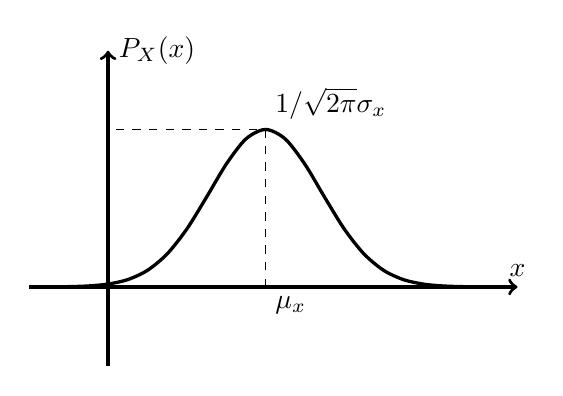
\begin{tikzpicture}[scale=2]
    \draw[->,very thick](-1.5,0)--(1.6,0)node[above]{$x$};
    \draw[->,very thick](-1,-0.5)--(-1,1.5)node[right]{$P_X(x)$};
    \node[below right]at(0,0){$\mu_x$};
    \draw[dashed](0,0)--(0,1)--(-1,1);
    \node[above right]at(0,1){$1/\sqrt{2\pi}\sigma_x$};


    \draw[-,very thick]plot[smooth, domain=-1.5:1.5](\x,{e^(-(2*\x)^2)});
\end{tikzpicture}
\end{document}